\documentclass[a4paper, 12pt, draft]{article}
\usepackage{blindtext}
%
\usepackage{geometry}
\geometry{
	showframe=true,
	includeheadfoot,
	ignoremp,
	vdivide={0.5cm,*,1cm},
	hdivide={1.5cm,*,1cm}
}
%
\usepackage{tikz}
\usetikzlibrary{backgrounds, calc, fadings}
\begin{document}
	Uso de la grid de backgrounds para ubicar las coordenadas y con calc ubicamos el punto medio de una ruta. También, a nivel visual usamos nodos dibujados con figuras geométricas.
	\begin{figure}[h]
		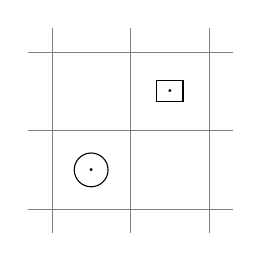
\begin{tikzpicture}[show background grid, loose background]
			\path (0,0)coordinate(a) -- (1,1)coordinate(b) -- (2,2)coordinate(c);
			\node[draw, circle] at ($(a)!0.5!(b)$){.};
			\node[draw, rectangle] at ($(b)!0.5!(c)$){.};
		\end{tikzpicture}
	\end{figure}
	Abordando algunos keywords de la fadings podemos ver draw opacity como un atenuador de las líneas dibujadas por draw.
	\begin{figure}[h]
		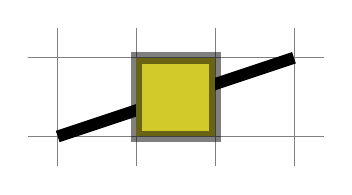
\begin{tikzpicture}[show background grid, loose background, line width=1ex]
			\draw (0,0) -- (3,1);
			\filldraw[fill=yellow!80!black, draw opacity=0.5] (1,0) rectangle (2,1);
		\end{tikzpicture}
	\end{figure}
	Así como opacity coloca la transparencia tanto para draw y fill, tambíen hay grados como lo serían con: transparent, ultra nearly transparent, very nearly transparent, nearly transparent, semitransparent, nearly opaque, very nearly opaque, ultra nearly opaque, opaque.
	\begin{figure}[h]
		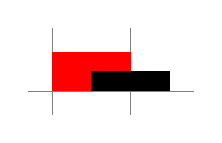
\begin{tikzpicture}[show background grid, loose background, line width=1ex]
			\fill[red] (0,0) rectangle (1,0.5);
			\fill[opaque] (0.5,0) rectangle (1.5,0.25);
		\end{tikzpicture}
	\end{figure}
	\blindtext
\end{document}